\section{Speculation}
\label{sec:speculation}
Whenever we move an instruction above a branch it is control-flow dependent on, we consider this instruction to be \textit{speculatively} executed~\cite{chang95}. When speculating during compilation, we typically try to tailor the control-flow of the program towards the actual behavior we expect during runtime. The most common types of speculations include loads, computations and stores. While these may increase performance in certain cases, they each come with considerations and hazards one has to be aware of. In this section, we will study the concepts and heuristics behind speculative execution. 


%% TODO Talk about [[likely]] / [[unlikely]] https://clang.llvm.org/docs/AttributeReference.html#likely-and-unlikely\textbf{}
\subsection{Example}
\begin{center}
    \begin{minipage}{.45\textwidth}
        \centering
        \begin{lstlisting}[style=CStyle]
if (x > 0) {
    y = array[x];
}
\end{lstlisting}
        \captionsetup{type=listing}
        \captionof{lstlisting}[Example Conditional Load]{Setting the value of \texttt{y} depends on \texttt{x} being positive.}
    \end{minipage}\hfill
    \begin{minipage}{.45\textwidth}
        \centering
        \begin{lstlisting}[style=CStyle]
int temp = array[x]; 
if (x > 0) {
  y = temp;
}
\end{lstlisting}
        \captionsetup{type=listing}
        \captionof{lstlisting}[Example Speculative Load]{We can speculatively load the value of \texttt{array[x]} into a additional variable.}
    \end{minipage}
\end{center}

\begin{center}
    \begin{minipage}{.45\textwidth}
        \centering
        \begin{lstlisting}[style=AsmStyle]
LDR     r3, [r0]        
CMP     r3, #0          
BLE     skip_load_and_store
LDR     r1, [r2, r3, LSL #2] 
STR     r1, [r4]
skip_load_and_store:
\end{lstlisting}
        \captionsetup{type=listing}
        \captionof{lstlisting}[Example Instructions Conditional Load]{Once we know the branch is not taken, we issue a load of \texttt{data[x] into \texttt{r1}}}
    \end{minipage}\hfill
    \begin{minipage}{.45\textwidth}
        \centering
        \begin{lstlisting}[style=AsmStyle]
LDR     r3, [r0]            
LDR     r1, [r2, r3, LSL #2]
CMP     r3, #0              
BLE     skip_store 
STR     r1, [r4]            
skip_store:
\end{lstlisting} 
        \captionsetup{type=listing}
        \captionof{lstlisting}[Example Instructions Speculative Load]{We immediately issue a load for \texttt{data[x]}, even tough we do not know yet if it will be needed.}
    \end{minipage}
\end{center}

\subsection{Superblock Structure}
If we consider the control flow of a program, a superblock~\cite{10.1145/161541.159765} is a consecutive sequence of instruction which is always entered at the top-most basic block but may be left at arbitrary and multiple points. When forming superblock, we try to anticipate the future control flow of the program during run time by either profiling it with synthetic data or other means~\cite{639244}. An example of how the profile of a loop execution may look like can be seen in figure~\ref{fig:controlflow_side_enterance}. Note that most iterations consist of BB2, BB3 and BB5. Blocks which are frequently executed together are also called traces. To create a superblock from this trace, we need to remove the side entrance from BB4 to BB5 and hence to the trace section. Typically, this done with tail duplication. In this case, we need to add BB5' to remove the side entrance, as can be seen in figure ~\ref{fig:controlflow_superblock}. By forming superblocks, we can avoid bookkeeping complexity which typically arises during trace scheduling when we move instructions across side entrances.
 Note that also BB4 and BB5' now form a superblock. Superblocks are not exclusively tools of speculation, rather they are also important for enabling other optimizations in compilers. 



% TODO Jakob: Add this figure
\begin{figure}[H]
        \centering
        \resizebox{0.73\textwidth}{!}{
            %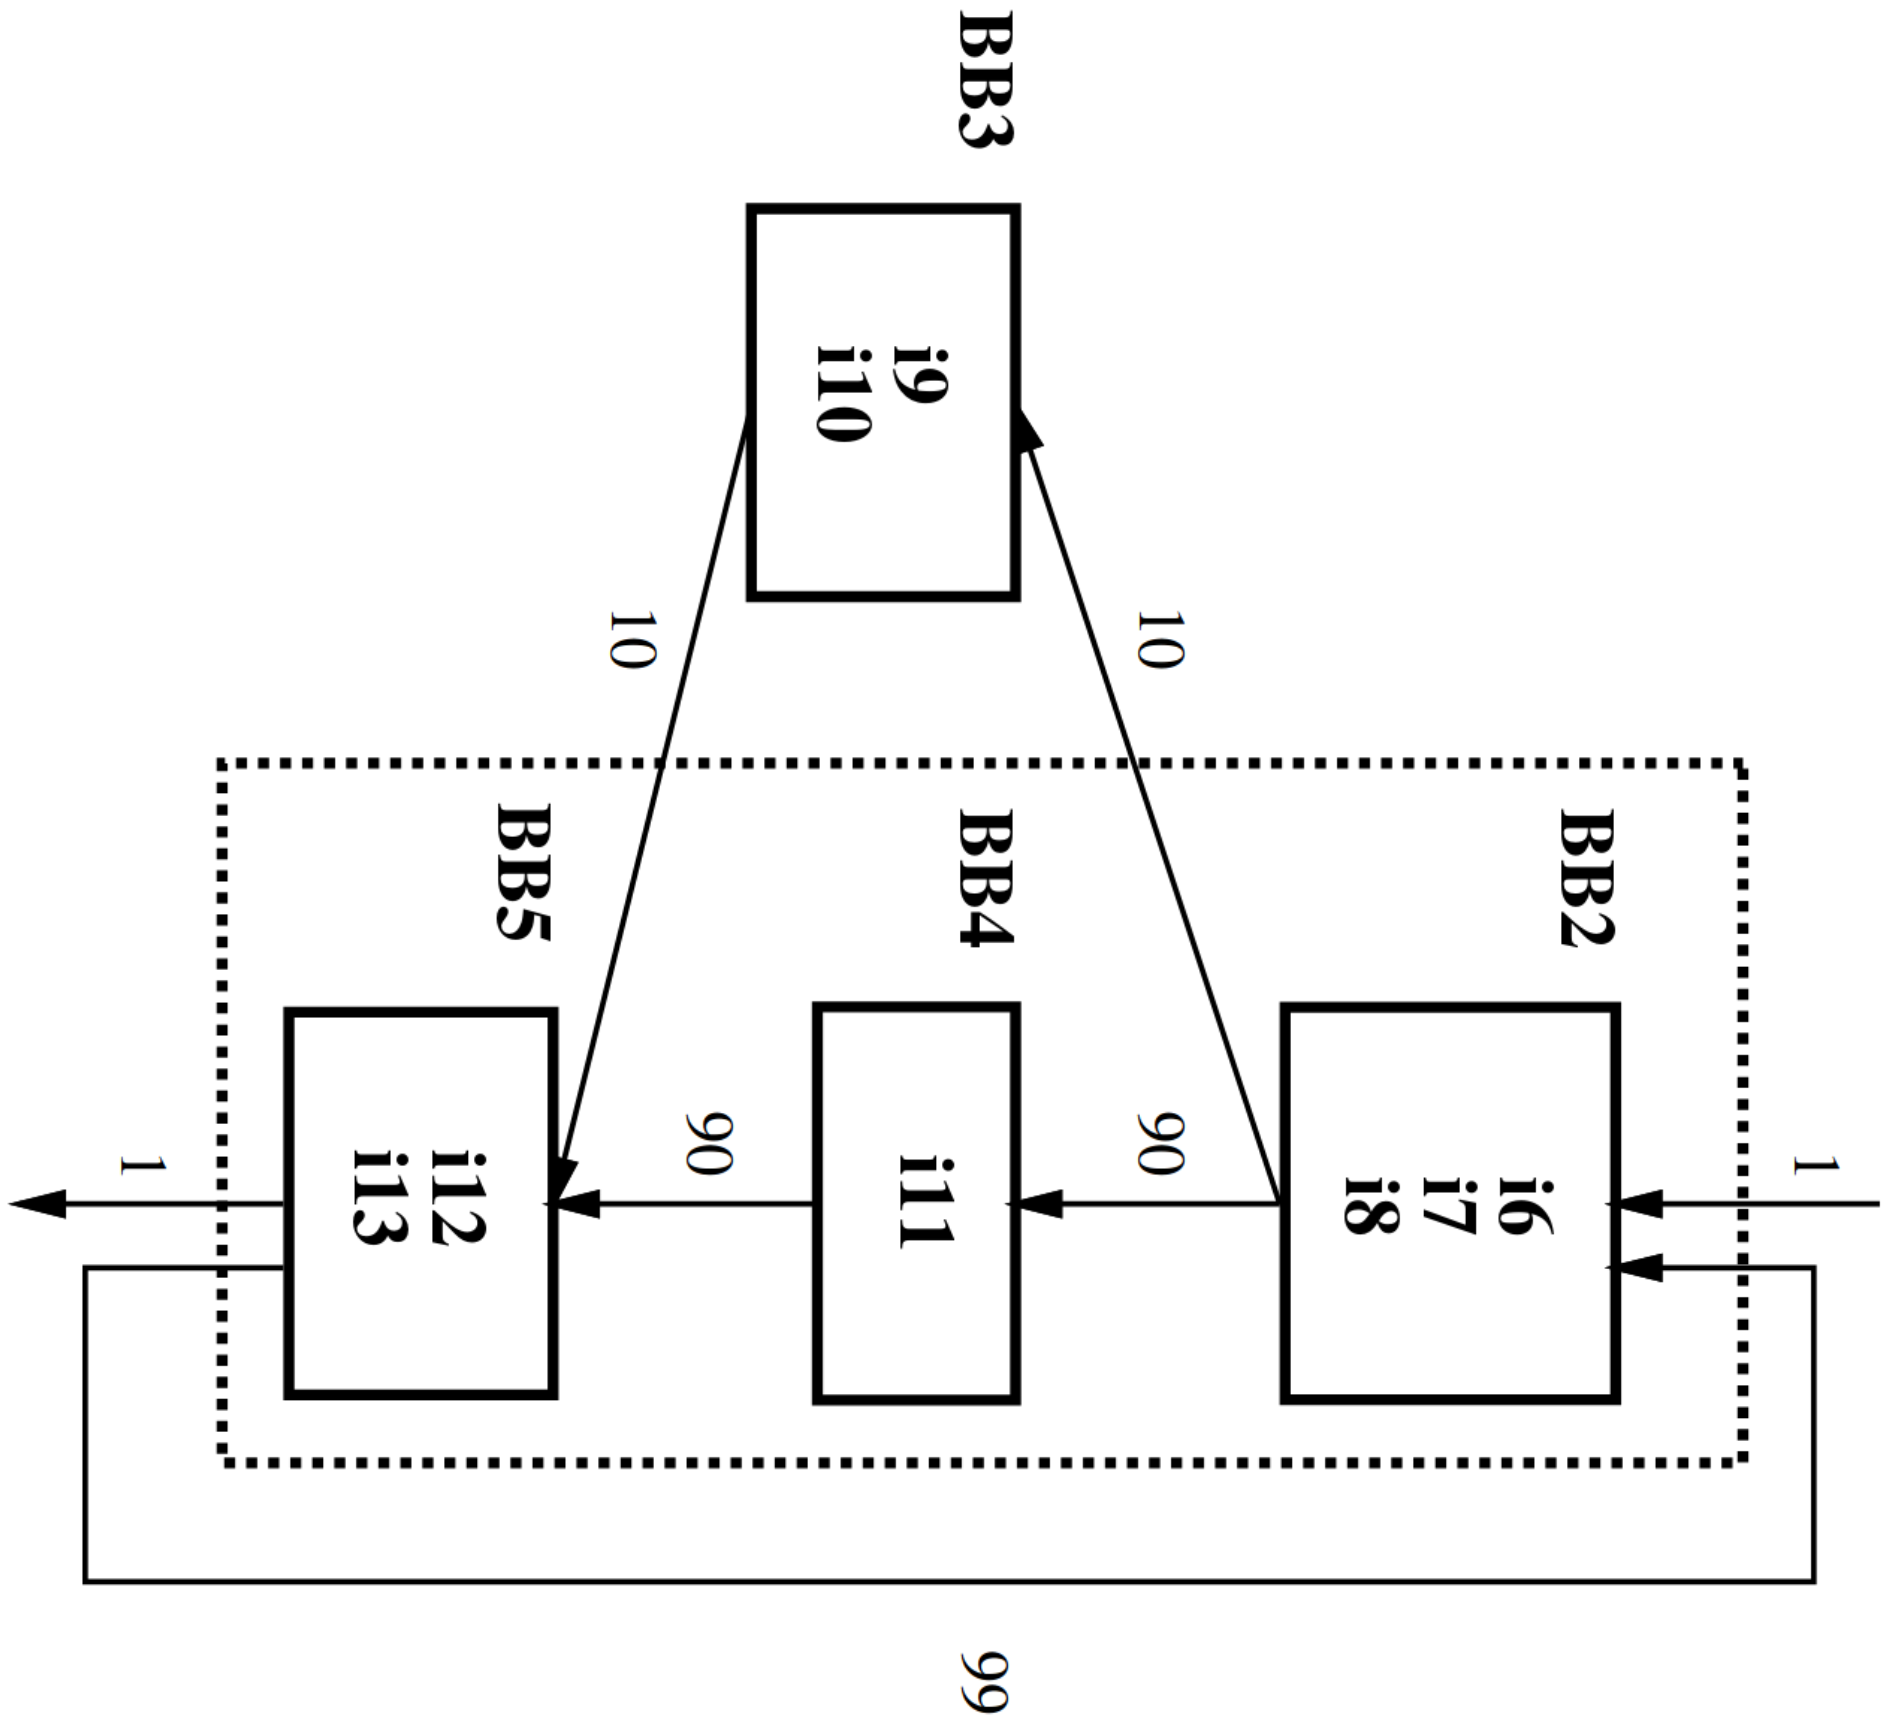
\includegraphics[width=\linewidth, angle=90]{src//figure//image/image_chang_loop_cfg.png}

             
\includegraphics[width=0.1\linewidth]{assets/placeholder.png}
        }
        \caption{Trace with Side Entrance}{The edge from BB4 to BB5 is a so-called side entrance into thew the most important trace consisting of BB2, BB3, and BB5.}
        \label{fig:controlflow_side_enterance}
\end{figure}

% TODO Jakob: Add this figure
\begin{figure}[H]
        \centering
        \resizebox{0.73\textwidth}{!}{
            %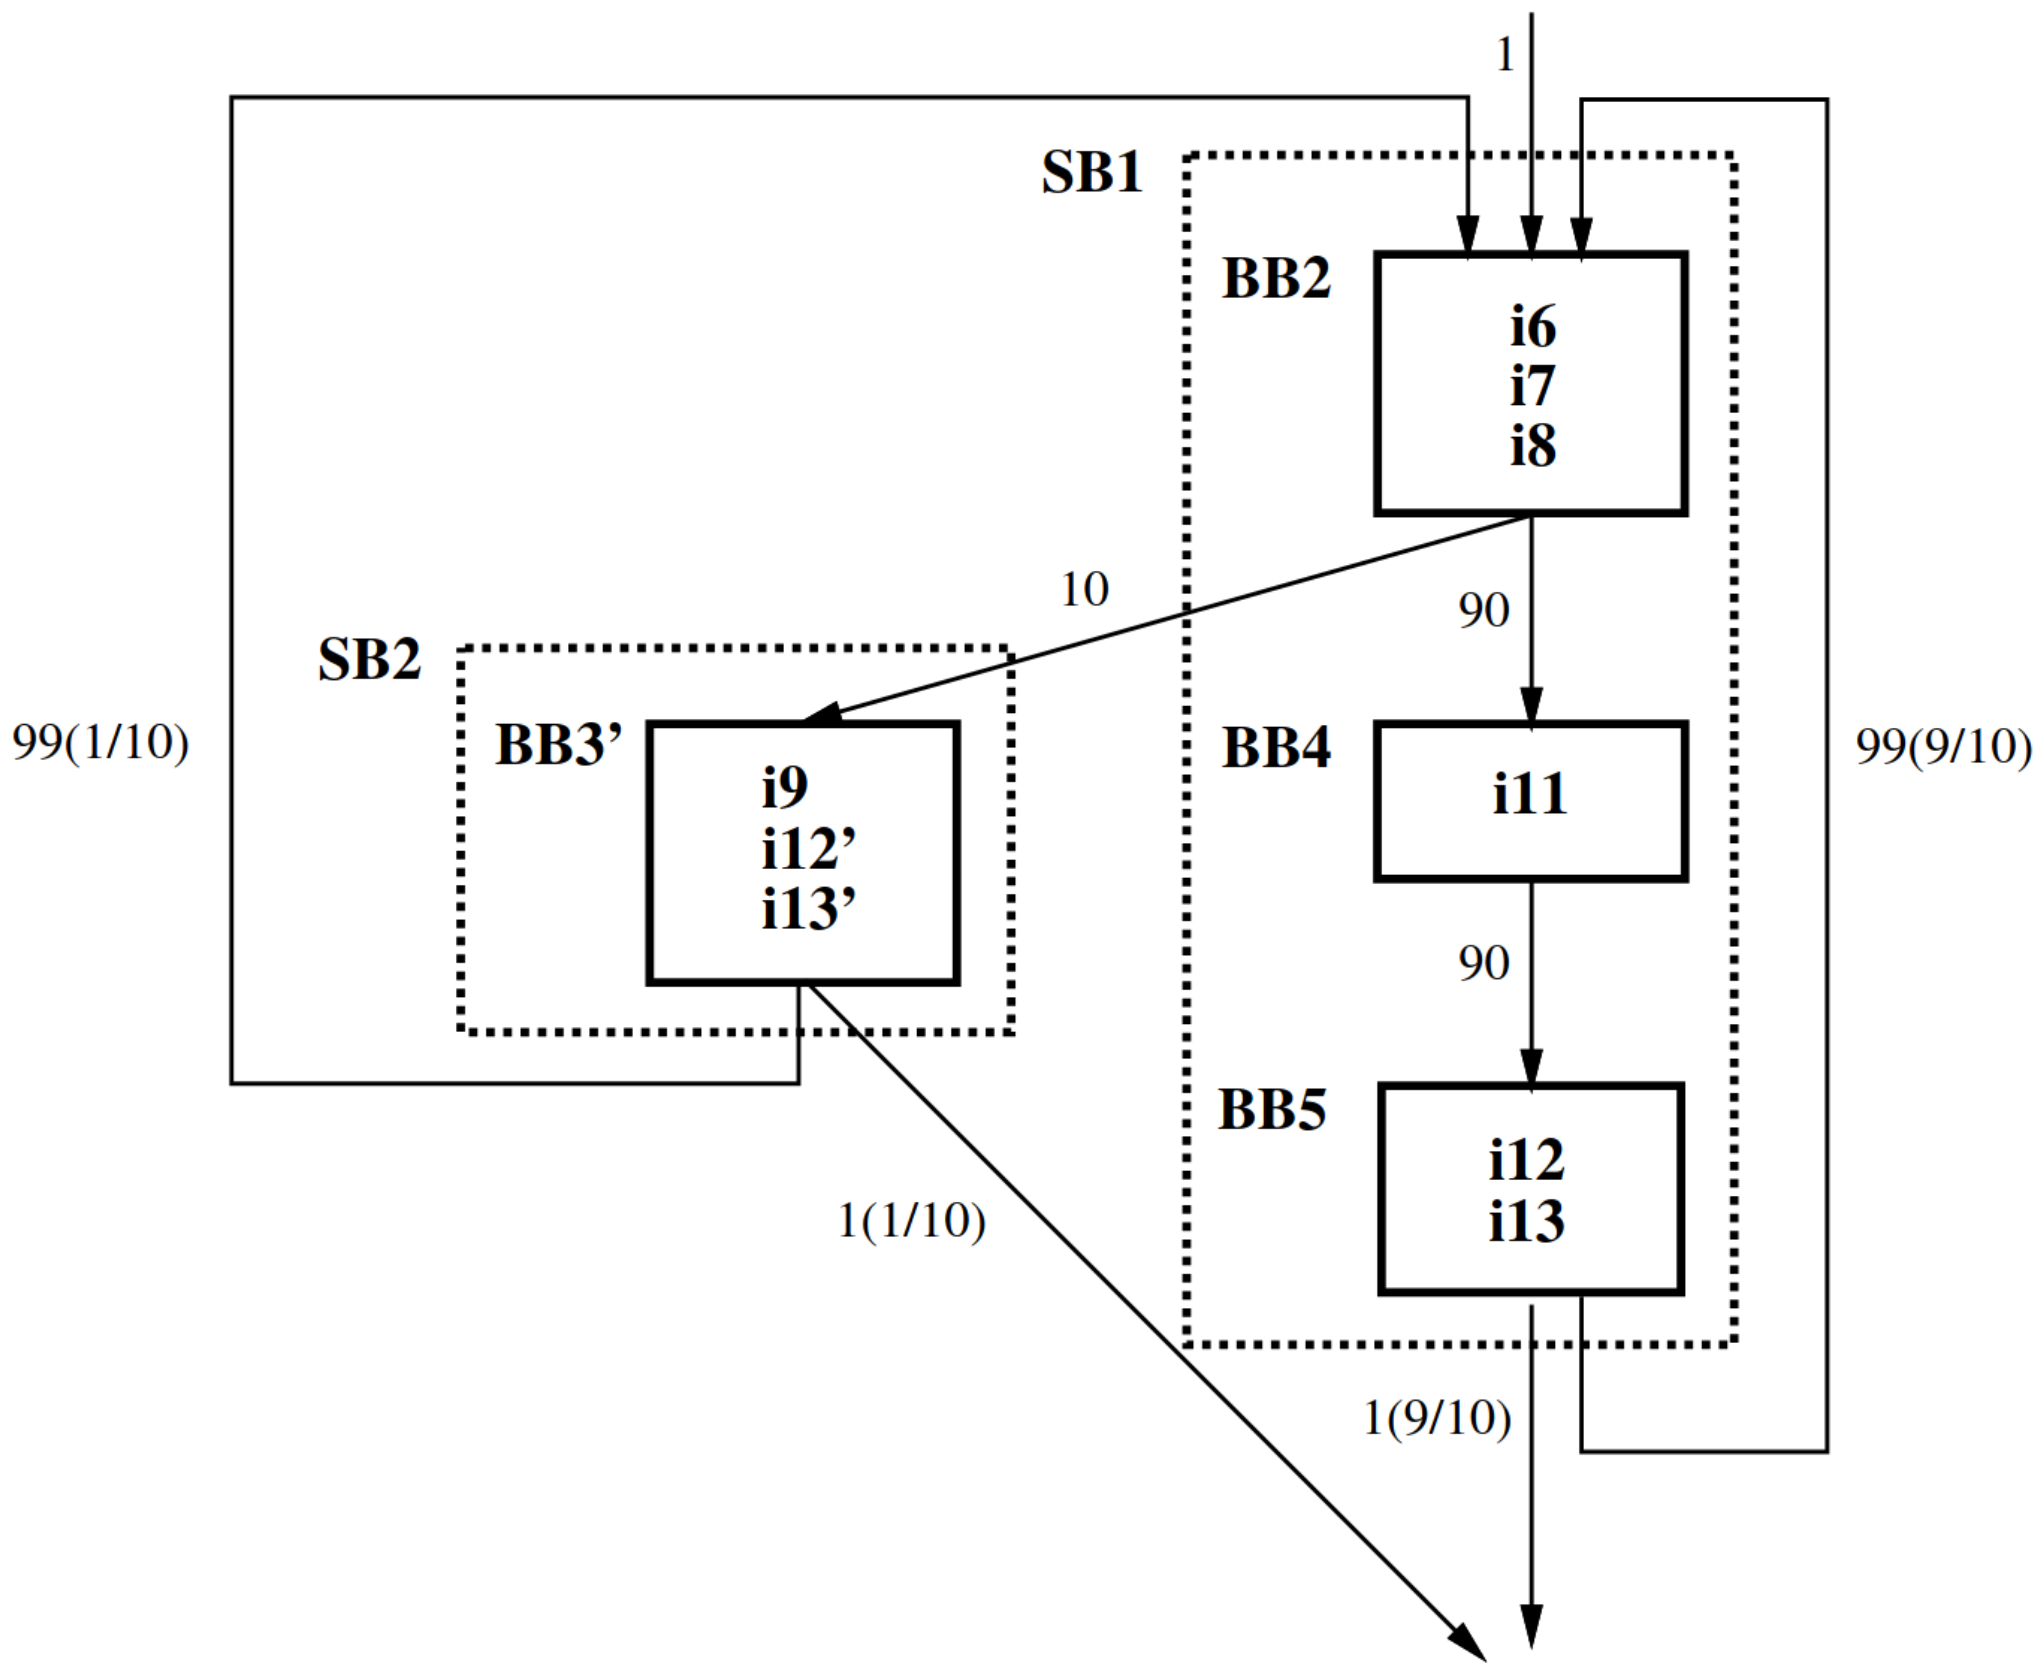
\includegraphics[width=0.5\linewidth]{src//figure//image/image_chang_sb_loop_cfg.png}

             
\includegraphics[width=0.1\linewidth]{assets/placeholder.png}
        }
        \caption{Superblock Example}{In this example, we removed the side entrance into the trace by duplicating BB5 (BB5') for the case where BB2 is branching to BB4.}
        \label{fig:controlflow_superblock}
\end{figure}

\subsection{Superblock Scheduling}
After the trace selection and the formation of superblocks, the compiler has to schedule the instructions with the goal of enabling as much ILP as possible and the constraint of producing a save and correct program. This is done by building a graph which represents the dependencies among the instructions. The dependency graph is used during and a subsequent list scheduling. The compiler may use heuristics and given instruction latencies to assign priorities to instructions which are \textit{ready} to produce a schedule which will use the available resources as efficient as possible~\cite{chang95}. To this end, the compiler needs to be able to move instructions above previous branches which is considered a speculation. 
%%% TODO 14.11. Jakob Explain benefits of SB and superblock scheduling 

\subsection{Speculative Code Motion Models}
In many cases, higher performance can be achieved by moving certain instructions either down or upward. However, in both cases we have to retain the correctness of the original program. A variable or register is called \textit{live} if it holds a value that will be needed by other instructions.  For branching instructions, we can define \texttt{live-out(Br)} as the set of variables which may be used before being defined in case \texttt{Br} will be taken. Downward code motion, meaning moving a instruction \texttt{I} beneath a later instruction \texttt{Br} can always be applied if \texttt{Br} is not dependent on the result of \texttt{I}. In case the destination register of \texttt{I} is in \texttt{live-out(Br)}, we have to insert a copy of \texttt{I} between \texttt{Br} and its target to insure correctness, as can be seen in listing~\ref{ls:ls_downward_default}

\begin{center}
    \begin{minipage}{.45\textwidth}
        \centering
        \begin{lstlisting}[style=AsmStyle]
    LDR     r1, [R2]
    CMP     r3, #0
    BEQ     Target
    ADD     r4, r1, r5
    ; ...
Target:
    SUB     r6, r1, r7
\end{lstlisting}
        \captionsetup{type=listing}
        \captionof{lstlisting}[Default Example Downward Motion]{Since \texttt{r1} is needed in the branch target of the \texttt{BEQ} instruction, \texttt{live-out(BEQ)} contains \texttt{r1}.}
        \label{ls:ls_downward_default}
    \end{minipage}\hfill
    \begin{minipage}{.45\textwidth}
        \centering
        \begin{lstlisting}[style=AsmStyle]    
    CMP     r3, #0
    BEQ     Target
    LDR     r1, [r2]
    ADD     r4, r1, r5
    ; ...
Target:
    @LDR     r1, [r2]@
    SUB     r6, r1, r7
\end{lstlisting}
        \captionsetup{type=listing}
        \captionof{lstlisting}[Downward Motion with Copy]{We can delay the \texttt{LDR} instruction by moving it downward. However, in case the \texttt{BEQ}-branch is taken, we need to load the correct value using a copy of the \texttt{LDR} instruction.}
    \end{minipage}
\end{center}

Although downward motion can be easily done, the cases where we will gain performance are limited. Moving an instruction from a point after a branch to a point before the branch is refereed to as upward motion. Typically, one may try to schedule long-latency instructions early to reduce the critical path, for example in a superblock. Similar to other architectures, the division instruction \texttt{SDIV} is a example of such a long-latency instruction. As can be seen in listing ~\ref{ls:ls_upward_default}, depending on the input data, we may have to execute \texttt{SDIV}. Therefore it would we preferable to speculatively execute the division as can be seen in listing~\ref{ls:ls_upward_faulty}. However, the destination of \texttt{SDIV} (\texttt{r1}) is in \texttt{live-out(BEQ)} if it is taken, hence the speculation would alter the result if the compiler does not introduce compensation code, e.g. a copy of \texttt{r1} for the \texttt{taken} case. Additionally, \texttt{SDIV} may cause an exception since it was moved above the branch which checks the loaded value in \texttt{r1} to be zero. 

\begin{center}
    \begin{minipage}{.45\textwidth}
        \centering
        \begin{lstlisting}[style=AsmStyle]    
    LDR r1, [address]
    CMP r1, #0
    BEQ taken
    SDIV r1, #5, r1
    B end
taken:
    ADD r1, r1, #2
end:
\end{lstlisting}
        \captionsetup{type=listing}
        \captionof{lstlisting}[Default Example Upward Motion]{Depending on the input data, we may have to execute a division which typically takes many cycles in most architectures.}
        \label{ls:ls_upward_default}
    \end{minipage}\hfill
    \begin{minipage}{.45\textwidth}
        \centering
        \begin{lstlisting}[style=AsmStyle]
    ldr r1, [address]
    ldr r2, [address2]
    @sdiv r2, #5, r1@
    beq taken, r1, #0
    b end
taken:
    add r1, r2, #2
end:
\end{lstlisting}
        \captionsetup{type=listing}
        \captionof{lstlisting}[Faulty Upward Motion ]{The long-latency division was naively moved upwards. Depending on the input data, the program will now compute wrong results, because the destination register of the speculatively executed division \texttt{r1} is in \texttt{live-out(BEQ)}. In addition, \texttt{SDIV} may cause a unnecessary a divide-by-zero exception.}
        \label{ls:ls_upward_faulty}
    \end{minipage}
\end{center}

\paragraph{Restriction 1:} The destination register of \texttt{I} is not part of \texttt{live-out(Br)}. Hence, the result of \texttt{I} is not used before it is redefined when the branch was taken.
\paragraph{Restriction 2:} Instruction \texttt{I} will not cause an exception which will alter the program execution if \texttt{Br} was taken. 


Restricted Percolation is a conservative code motion technique where the compiler moves instructions across basic blocks or control-flow boundaries under strict safety conditions. Instructions are only moved when it is guaranteed that such movement will not alter the program's observable behavior. Minimal or no speculation is involved, and the movement is based on provable safety. The technique strictly respects data dependencies (ensuring that an instruction's operands are ready) and control dependencies (ensuring the instruction is only executed when it should be).
